\documentclass[11pt]{article}
\usepackage[a5paper,margin=14mm]{geometry}
\usepackage{fontspec}
\setmainfont{TeX Gyre Termes}
\setsansfont{TeX Gyre Heros}
\usepackage{amsmath}
\usepackage{tikz}
\usetikzlibrary{arrows.meta,calc,positioning,shapes.geometric,fit,backgrounds,decorations.pathmorphing,matrix}

\begin{document}
\section*{Pipeline diagram}
\begin{center}
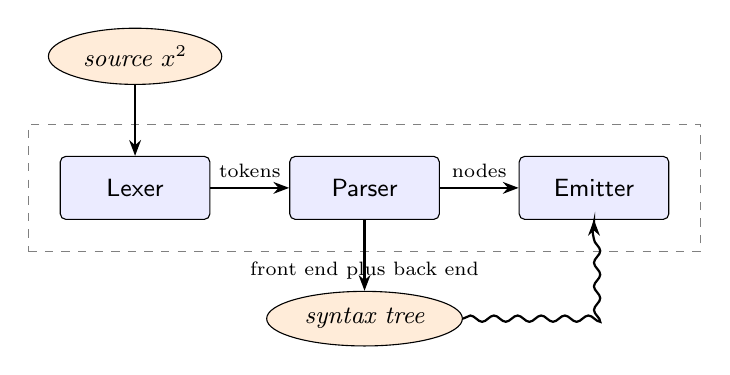
\begin{tikzpicture}[
  node distance=9mm and 10mm,
  stage/.style={draw,rounded corners=2pt,fill=blue!8,minimum width=19mm,minimum height=8mm,font=\sffamily\small},
  data/.style={draw,ellipse,fill=orange!15,font=\small\itshape},
  flow/.style={-{Stealth[length=2mm]},thick}]
  \node[stage] (lex) {Lexer};
  \node[stage,right=of lex] (par) {Parser};
  \node[stage,right=of par] (gen) {Emitter};
  \node[data,below=of par] (ast) {syntax tree};
  \node[data,above=of lex] (src) {source $x^2$};
  \draw[flow] (lex) -- node[above,font=\scriptsize]{tokens} (par);
  \draw[flow] (par) -- node[above,font=\scriptsize]{nodes} (gen);
  \draw[flow] (par) -- (ast);
  \draw[flow] (src) -- (lex);
  \draw[flow,decorate,decoration={snake,amplitude=.4mm,segment length=3mm}] (ast.east) -| (gen.south);
  \begin{scope}[on background layer]
    \node[draw=gray,dashed,fit=(lex)(par)(gen),inner sep=4mm,label={[font=\scriptsize]below:front end plus back end}] {};
  \end{scope}
\end{tikzpicture}
\end{center}

\section*{Geometry with calc}
\begin{center}
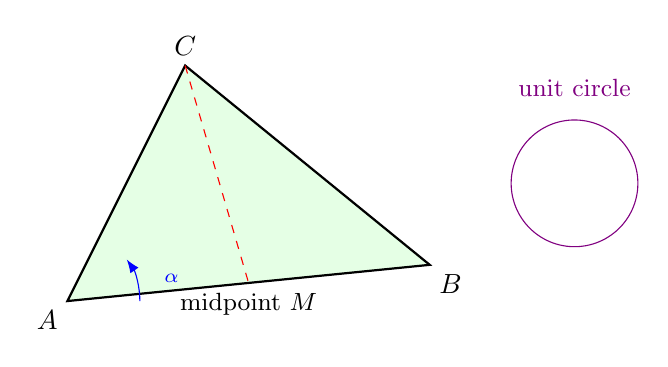
\begin{tikzpicture}[scale=1.15]
  \coordinate (A) at (0,0);
  \coordinate (B) at (4,0.4);
  \coordinate (C) at (1.3,2.6);
  \draw[thick,fill=green!10] (A) -- (B) -- (C) -- cycle;
  \coordinate (M) at ($(A)!0.5!(B)$);
  \draw[red,dashed] (C) -- (M);
  \node[below left] at (A) {$A$};
  \node[below right] at (B) {$B$};
  \node[above] at (C) {$C$};
  \node[below,font=\small] at (M) {midpoint $M$};
  \draw[blue,-{Latex}] (A) ++(0.8,0) arc[start angle=0,end angle=35,radius=0.8];
  \node[blue,font=\scriptsize] at (1.15,0.25) {$\alpha$};
  \draw[domain=0:360,samples=60,smooth,variable=\t,violet] plot ({5.6+0.7*cos(\t)},{1.3+0.7*sin(\t)});
  \node[violet,font=\small] at (5.6,2.35) {unit circle};
\end{tikzpicture}
\end{center}

\section*{Matrix of nodes}
\begin{center}
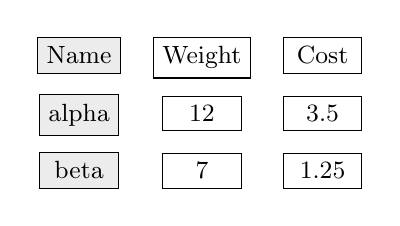
\begin{tikzpicture}
  \matrix[matrix of nodes,row sep=2mm,column sep=4mm,nodes={draw,minimum width=10mm,font=\small},
          column 1/.style={nodes={fill=gray!15}}]{
    Name & Weight & Cost\\
    alpha & 12 & 3.5\\
    beta & 7 & 1.25\\
  };
\end{tikzpicture}
\end{center}
\end{document}
